\documentclass[../Article_Model_Parameters.tex]{subfiles}
\graphicspath{{\subfix{../Figures/}}}
\begin{document}
	
	Supercritical CO$_2$ is defined as carbon dioxide that is pressurized and heated above its critical point (31.1 $^\circ C$, 74 bar). Depending on the operating conditions, the fluid properties such as viscosity and density can vary, which leads to multiple industrial applications of CO$_2$.
	
	The supercritical carbon dioxide is commonly used for impregnation as described by \citet{Weidner2018}, \citet{Machado2022} or \citet{Fathi2022}. Impregnation is defined as modifying the properties of bulk substances by physically or chemically binding/adsorbing impregnates to a bulk material or surface, such as the hydrophobization of surfaces. The main advantage of using supercritical CO$_2$ is that after depressurization, it desorbs from the surface and evaporates, leaving a solvent-free product. On the other hand, the main disadvantage of using carbon dioxide for impregnation is the low solubility of many drugs of interest.
	
	Another application of supercritical CO$_2$ is nanoparticles formation as investigated by \citet{Padrela2018}, \citet{Franco2021}, \citet{SaadatiArdestani2020} or \citet{Sodeifian2022}. Supercritical carbon-dioxide-assisted technologies enable the production of different morphologies of different sizes, including nanoparticles and nanocrystals, by modulating operating conditions. Supercritical fluid-based processes have advantages over techniques conventionally employed to produce nanosized particles or crystals, such as reduced use of toxic solvents. Moreover, the CO$_2$ is completely removed from the final product by simple depressurization.
	
	One of the most popular applications of supercritical CO$_2$ is the extraction of essential oils, as described by many researchers, for example, by \citet{Sodeifian2017}, \citet{Reverchon1993} or \citet{Sovova1994}. Traditional methods, such as distillation and organic solvent extraction, are commonly employed but have drawbacks. Distillation, involves high temperatures that can lead to the thermal degradation of heat-sensitive compounds. This limitation has increased the popularity of alternative techniques, such as supercritical fluid extraction. Supercritical CO$_2$ is appealing due to its distinctive properties: it is inflammable, non-toxic and non-corrosive. Supercritical fluids can exhibit both gas- and liquid-like properties, allowing for adjustable dissolving power through changes in operating conditions. 
	
	This study investigates the extraction of essential oil from chamomile flowers (Matricaria chamomilla L.) via supercritical fluid extraction techniques and the modelling of this process. Chamomile is a medicinal herb widely cultivated in southern and eastern Europe — in countries such as Germany, Hungary, France and Russia. It can be found outside Europe, for instance in Brazil as discussed by \citet{Singh2011}. This plant is distinguished by its hollow, bright gold cones, housing disc or tubular florets and surrounded by about fifteen white ray or ligulate florets. Chamomile has been used for its medicinal benefits, serving as an anti-inflammatory, antioxidant, mild astringent, and healing remedy. Extracts of chamomile are widely used to calm nerves and mitigate anxiety, hysteria, nightmares, insomnia and other sleep-related conditions, according to \citet{Srivastava2009}. \citet{Orav2010} reported that oil yields from dried chamomile samples ranged from 0.7 to 6.7 mL/kg. The highest yields of essential oil, between 6.1 and 6.7 mL/kg, were derived from chamomile sourced from Latvia and Ukraine. In comparison, chamomile from Armenia exhibited a lower oil content of 0.7 mL/kg.
	
	The literature offers various mathematical models to describe the extraction of valuable compounds from biomass. Selecting a process model is case-to-case dependent and requires analysis of each model's specific assumptions about mass transfer and thermodynamic equilibrium.
	
	\citet{Goto1996} presented the Shrinking Core (SC) model, which describes a process of irreversible desorption that is followed by diffusion through the pores of a porous solid. When the mass transfer rate of the solute in the non-extracted inner region is significantly slower than in the outer region, where most of the solute has already been extracted, or when the solute concentration exceeds its solubility in the solvent, a distinct boundary may form between the inner and outer regions. As extraction progresses, the core of the inner region shrinks. The model envisions supercritical CO$_2$ extraction as a sharp, inward-moving front, with a completely non-extracted core ahead of the front and a fully extracted shell behind it.
	
	\citet{Sovova1994} proposed The Broken-and-Intact Cell (BIC) model, which assumes that a portion of the solute, initially stored within plant structures and protected by cell walls, is released during the mechanical breakdown of the material. The solute located in the region of broken cells near the particle surface is directly exposed to the solvent, while the core of the particle contains intact cells with undamaged walls. This model describes three extraction phases: a fast extraction phase for accessible oil, a transient phase, and a slow phase controlled by diffusion. The model has been successfully applied to the extraction of grape oil (\citet{Sovova1994b}) and caraway oil (\citet{Sovova1994a}).
	
	The Supercritical Fluid Extraction (SFE) process can be be treated similarly to heat transfer, considering solid particles like hot balls cooling down in a uniform environment. \citet{Bartle1990} introduced the hot ball diffusion (HBD) model, where spherical particles with uniformly distributed solute diffuse similarly to heat diffusion. Unlike the BIC model, where solute is readily available on the particle surface, the HBD model is suited for systems with small quantities of extractable materials and is not limited by solubility. The model is particularly relevant when internal diffusion controls mass transfer, allowing results from single particles to be extended to the entire bed under uniform conditions. \citet{Reverchon1993} have further elaborated on the HBD model and used it to simulate extraction processes for natural materials.
	
	\citet{Reverchon1996} proposed a model for extraction of essential oils, which are mainly located inside the vegetable cells in organules called vacuoles. Only a small fraction of essential oil might be near the particle surface due to the breaking up of cells during grinding or in epidermal hairs located on the leaf surface. The fraction of oil freely available on the particle surface should not be significant in the case of SFE from leaves. Consequently, SFE of essential oil from leaves should be mainly controlled by the internal mass-transfer resistance. Therefore, the external mass-transfer coefficient was neglected in the development of the model of \citet{Reverchon1996}. The mass balances were developed in the additional hypotheses that the axial dispersion can be neglected and that the solvent density and flow rate are constant along the bed.
	
	This work builds upon the linear kinetic model suggested by \citet{Reverchon1996}, deriving fundamental governing equations to develop a comprehensive model for the chamomile oil extraction process. This model aims for control-oriented simplicity, assuming a semi-continuous operation within a cylindrical vessel. The process involves a supercritical solvent being pumped through a fixed bed of finely chopped biomass to extract the solute, followed by separation of the solvent and solute in a flush drum to collect the extract. Parameters such as pressure ($P$), feed flow rate ($F$) and inlet temperature ($T^{in}$) are adjustable and measurable, while the outlet temperature ($T^{out}$) and the amount of product at the outlet can only be monitored. Figure \ref{fig: SFE_drawing} presents a simplified process flow diagram.
	
	\begin{figure}[!ht]
		\centering
		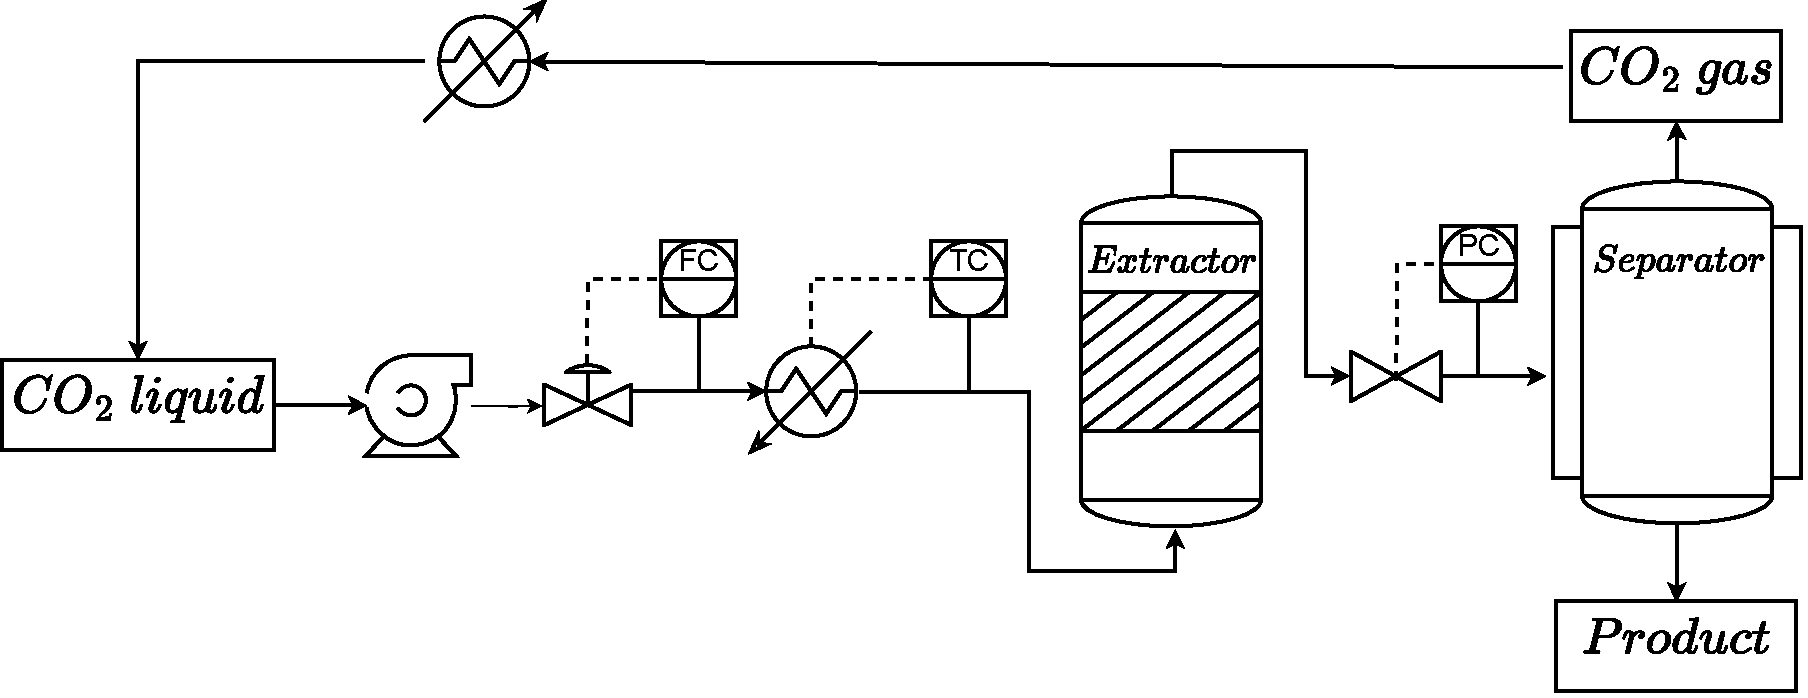
\includegraphics[width=\columnwidth]{Figures/PFD.drawio.pdf}
		\caption{Process flow diagram}
		\label{fig: SFE_drawing}
	\end{figure}
	
\end{document}